\scanpage{44}

\margin{\handwritten{\deleted{\unsure{XVI|XII}} 5.2}}

$\operatorname{Et}(Z)$\quad ($Z$ , schéma)\quad XII 5.9

\figure{\begin{tikzpicture}[x=1cm,y=1cm]
\draw (1.20,.50) .. controls (.45,.72) and (-1.35,.58) .. (-1.43,.00) .. controls (-1.48,-.42) and (-.72,-.53) .. (-.05,-.45);
\end{tikzpicture}}

Chow (lemme de - )\quad Chow lemma\quad XII 7.1

\deleted{Lemme de Chow}

\unsure{\deleted{t}T|\deleted{E}T|\deleted{T}E|T}héorè\unsure{\deleted{p}m|\deleted{m}p}e de finitude \deleted{pour un morphisme propre\quad finiteness theorem for a}\inserted{finiten\unsure{\deleted{p}e|\deleted{e}p}ss theorem}\quad \handwritten{$\overline{\underline{\mathrm{\unsure{XIV|XVI}}}}$ 1.1, \deleted{\unsure{XVI 5.3|XVI 5.1}}\inserted{$\overline{\underline{\mathrm{XVI}}}$ 5.1, 5.2} XVII ...) \inserted{$\overline{\underline{\mathrm{XIX}}}$ 5.1}}

\figure{\begin{tikzpicture}[x=1cm,y=1cm]
\draw[line width=.50pt] (-2.55,.57) .. controls (-2.65,.20) and (-2.45,.10) .. (-2.16,.03) .. controls (-2.01,-.03) and (-1.99,-.30) .. (-2.04,-.57) .. controls (-2.10,-.33) and (-2.10,-.08) .. (-1.98,.01) .. controls (-1.60,.19) and (-.76,.03) .. (.05,.15) .. controls (.65,.19) and (1.00,.29) .. (1.04,.72);
\draw[line width=.32pt] (1.48,.71) .. controls (1.26,.27) and (1.36,.11) .. (1.80,.04) .. controls (2.22,-.01) and (2.62,-.03) .. (2.78,-.31);
\draw[line width=.42pt] (2.59,-.50) -- (3.24,.34);
\end{tikzpicture}}

\deleted{\handwritten{a)} pour morphisme propre\quad XIV 1.1}

\deleted{proper morphism\quad XIV 1.1}

\deleted{\handwritten{b)} pour $R^i_{\handwritten{!}}f$\quad XVII ...}

\margin{\handwritten{$\times$}}

\deleted{\handwritten{c)} pour un morphisme de type fini de schéma excellents\quad XIX 5.1}

\inserted{\handwritten{$\delta(x),\delta(F)$}}\quad $d(x)$

\figure{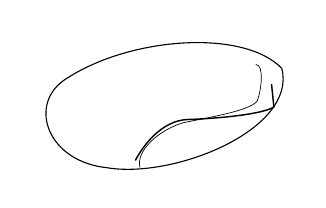
\begin{tikzpicture}[x=1cm,y=1cm]
\draw (1.35,.47) .. controls (.86,.98) and (-.62,.87) .. (-1.43,.31) .. controls (-1.87,-.02) and (-1.61,-.71) .. (-.88,-.79) .. controls (-.02,-.94) and (1.55,-.30) .. (1.35,.47);
\draw[line width=.25pt] (1.02,.52) .. controls (1.13,.52) and (1.09,.19) .. (1.04,.06) .. controls (.96,-.07) and (.38,-.16) .. (.10,-.22) .. controls (-.21,-.31) and (-.51,-.58) .. (-.45,-.79);
\draw[line width=.52pt] (1.22,.27) -- (1.25,-.02) .. controls (1.09,-.12) and (.48,-.17) .. (.14,-.18) .. controls (-.17,-.20) and (-.40,-.49) .. (-.51,-.70);
\end{tikzpicture}}

($x$, point d'un schéma\deleted{\unsure{)|X|s}}, \inserted{$F$ faisceau \deleted{sur $X$}}\handwritten{)}\quad \deleted{XIV (2.1)}\quad XIV 2

\inserted{\handwritten{Lefschetz}} \handwritten{(}théorème de \deleted{Lefschetz}\inserted{\handwritten{-}} affine\handwritten{)}\quad affine Lefschetz theorem\quad XIV \handwritten{3}.1 \handwritten{, XIX 6,1}

\figure{\begin{tikzpicture}[x=1cm,y=1cm]
\draw[line width=.42pt] (.35,.58) .. controls (.35,.19) and (-.40,.05) .. (-.66,-.28) .. controls (-.80,-.44) and (-.83,-.57) .. (-.84,-.64);
\end{tikzpicture}}

Morphisme \inserted{(universellement)} $n$-acyclique ($n$, entier)\quad \inserted{(universally)} $n$-acyclic morphisme\quad XV 1.3, 1.7

\figure{\begin{tikzpicture}[x=1cm,y=1cm]
\draw[line width=.40pt] (0,.38) .. controls (-.07,.07) and (.12,.02) .. (.85,.04) -- (.91,-.40) -- (.95,-.03) .. controls (1.75,.10) and (3.40,.04) .. (3.82,.14) .. controls (4.00,.19) and (4.05,.28) .. (4.10,.39);
\draw[line width=.45pt] (5.90,.40) .. controls (6.05,.20) and (6.35,.13) .. (6.39,-.37) .. controls (6.42,-.03) and (6.48,.10) .. (6.74,.13) .. controls (7.60,.15) and (8.64,.08) .. (8.96,.14) .. controls (9.15,.18) and (9.17,.28) .. (9.18,.39);
\end{tikzpicture}}

\deleted{Morphisme universellement $n$-acyclique\quad universally acyclic morphism}

\margin{\handwritten{(\quad)}}

\margin{\figure{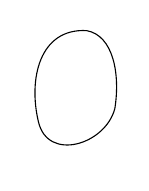
\begin{tikzpicture}[x=1cm,y=1cm]
\draw (.13,.76) .. controls (-.47,.79) and (-.61,.14) .. (-.48,-.40) .. controls (-.36,-.91) and (.37,-.69) .. (.49,-.23) .. controls (.56,.21) and (.47,.70) .. (.13,.76);
\end{tikzpicture}}}

morphisme \inserted{(universellement\unsure{\deleted{a}|\deleted{à}|à})} 1-asphérique\quad \deleted{(universellement)}\inserted{(universally) 1-aspheric} morphism\quad XV 1.7

\figure{\begin{tikzpicture}[x=1cm,y=1cm]
\draw[line width=.42pt] (0,.47) .. controls (-.13,.10) and (-.08,-.02) .. (.28,-.03) .. controls (.75,-.04) and (1.25,.01) .. (1.57,-.08) .. controls (1.86,-.14) and (1.97,-.46) .. (2.00,-.69) .. controls (2.00,-.26) and (2.06,-.18) .. (2.43,-.15) .. controls (3.15,-.08) and (4.28,-.22) .. (5.14,-.18) .. controls (5.34,-.17) and (5.36,.04) .. (5.33,.43);
\end{tikzpicture}}

\figure{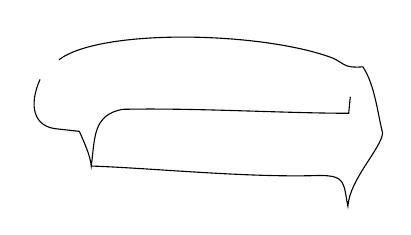
\begin{tikzpicture}[x=1cm,y=1cm]
\draw[line width=.40pt] (-.95,.45) .. controls (-1.10,.11) and (-1.03,-.16) .. (-.72,-.18) -- (-.45,-.21) .. controls (-.39,-.35) and (-.31,-.52) .. (-.30,-.65) .. controls (-.25,-.31) and (-.29,.00) .. (.10,.07) .. controls (1.00,.09) and (2.17,.02) .. (2.97,.02) -- (2.99,.23);
\draw[line width=.40pt] (-.71,.70) .. controls (-.18,1.10) and (1.87,1.06) .. (2.77,.72) .. controls (2.92,.65) and (2.91,.59) .. (3.15,.61) .. controls (3.30,.38) and (3.33,.06) .. (3.40,-.23) .. controls (3.39,-.42) and (2.98,-.82) .. (2.96,-1.16) .. controls (2.90,-.87) and (2.94,-.77) .. (2.60,-.77) .. controls (1.70,-.80) and (.52,-.68) .. (-.30,-.65);
\end{tikzpicture}}

\figure{\begin{tikzpicture}[x=1cm,y=1cm]
\draw (0,.61) .. controls (-.02,.44) and (.08,.39) .. (.01,.31) .. controls (-.23,.09) and (-.29,-.15) .. (-.20,-.43);
\end{tikzpicture}}

\deleted{morphisme universellement 1-asphérique\quad universally 1-aspheric morphism}

Morphisme \inserted{(\unsure{\deleted{t}u|\deleted{u}t}niversellement)} localement $n$-acyclique\quad \inserted{(universally)} locally $n$-acyclic morphism\quad XV 1.11

\figure{\begin{tikzpicture}[x=1cm,y=1cm]
\draw[line width=.30pt] (0,-.42) .. controls (-.03,-.14) and (.04,.13) .. (.24,.17) .. controls (1.10,.24) and (2.40,.14) .. (3.25,.13) .. controls (3.45,.12) and (3.51,.20) .. (3.53,.45);
\draw[line width=.30pt] (5.93,-.43) .. controls (5.88,-.16) and (5.98,.07) .. (6.19,.10) .. controls (6.97,.28) and (7.78,.04) .. (8.70,.08) .. controls (8.94,.09) and (9.01,.18) .. (8.99,.40);
\end{tikzpicture}}

morphisme \inserted{(universellement)} localement 1-asphérique\quad \inserted{(universally)} locally \deleted{\unsure{n|1}}\handwritten{1}-aspheric morphism\quad XV 1.11

\figure{\begin{tikzpicture}[x=1cm,y=1cm]
\draw[line width=.30pt] (0,-.48) .. controls (-.04,-.16) and (.04,.12) .. (.23,.16) .. controls (1.12,.10) and (2.49,.11) .. (3.20,.17) .. controls (3.48,.18) and (3.54,.25) .. (3.51,.45);
\draw[line width=.30pt] (5.90,-.46) .. controls (5.87,-.18) and (5.99,.06) .. (6.18,.08) .. controls (6.95,.24) and (8.08,.02) .. (8.54,.09) .. controls (8.93,.14) and (9.03,.26) .. (9.02,.46);
\end{tikzpicture}}

$A\handwritten{\unsure{\{\!\{|\{}}t\handwritten{\unsure{\}|\}\!\}}}$\qquad XV \handwritten{2}\deleted{\unsure{.|x|X}}\handwritten{.3.}

\figure{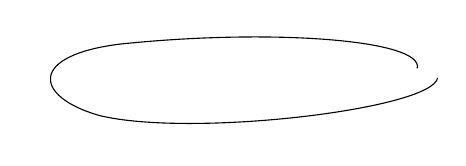
\begin{tikzpicture}[x=1cm,y=1cm]
\draw (2.33,.24) .. controls (2.42,.60) and (.50,.75) .. (-1.43,.55) .. controls (-2.61,.41) and (-2.55,-.12) .. (-1.70,-.36) .. controls (-.54,-.64) and (2.52,-.28) .. (2.59,.12);
\end{tikzpicture}}

théorème de changement de base par morphisme lisse\quad base change theorem \deleted{for} \unsure{\deleted{b}f|\deleted{f}b}or smooth base change\quad XVI 1.2

théorème de spécialisation pour la cohomologie\quad speciali\unsure{\deleted{s}z|\deleted{z}s}ation theorem for cohomology\quad XVI 2.2

théorème de pureté cohomologique relatif\quad relative purity theorem for cohomology\quad XVI 3.6, \inserted{3.7}

\figure{\begin{tikzpicture}[x=1cm,y=1cm]
\draw[line width=.44pt] (.09,.69) .. controls (-.39,.48) and (-.43,.12) .. (-.08,-.02) .. controls (.37,-.25) and (1.22,-.17) .. (1.62,-.50) .. controls (1.85,-.70) and (1.85,-.97) .. (1.83,-1.18) .. controls (2.02,-.89) and (2.18,-.66) .. (2.31,-.40);
\end{tikzpicture}}

théorème de pureté cohomologique absolue\quad absolute purity theorem for cohomology\quad XVI 3.9,XIX \inserted{1.2,2.1,3.2}

\figure{\begin{tikzpicture}[x=1cm,y=1cm]
\draw[line width=.42pt] (.35,.61) .. controls (.22,.69) and (.38,.69) .. (.54,.70) .. controls (1.80,.72) and (3.66,.92) .. (4.57,.75) .. controls (4.88,.69) and (5.02,.64) .. (5.06,.37) .. controls (5.16,.03) and (5.22,-.18) .. (5.08,-.43) .. controls (4.88,-.74) and (4.55,-1.02) .. (4.38,-1.19) .. controls (4.20,-1.36) and (4.21,-1.51) .. (4.26,-1.49) .. controls (4.43,-1.28) and (4.38,-1.05) .. (4.29,-.83) .. controls (4.18,-.47) and (3.75,-.45) .. (3.20,-.40) .. controls (1.76,-.30) and (.54,-.32) .. (.04,-.10) .. controls (-.19,.02) and (-.06,.33) .. (.10,.43);
\end{tikzpicture}}

couple lisse \inserted{de schémas relatifs}\quad smooth pair of relative schemes\quad XVI 3.1

\figure{\begin{tikzpicture}[x=1cm,y=1cm]
\draw[line width=.35pt] (0,-.42) .. controls (.03,-.05) and (.12,.10) .. (.44,.12) .. controls (.81,.08) and (1.37,.24) .. (2.15,.23) .. controls (2.94,.24) and (3.55,.15) .. (3.91,.25) .. controls (4.13,.29) and (4.18,.36) .. (4.14,.51);
\end{tikzpicture}}

\deleted{Lemme} Abhyankar (lemme d'\deleted{\unsure{A|)}} - relatif )\quad relative Anhyankar's lemma\quad XVI 3.5

théorème de comparaison pour les schémas algébriques sur $\underline{C}$\quad comparison theorem for algebraic schemes over $\underline{C}$\quad XVI 4.1

% archive sheet number: 43
